\documentclass[11pt]{article}
\usepackage{graphicx}
\usepackage{amsthm}
\usepackage{latexsym}
\usepackage{amssymb}
\usepackage{amsmath}
\usepackage{listings}
\usepackage[usenames]{color}
\lstset{language=Java}
\definecolor{CommentColor}{rgb}{0,0.45,0.08} 
\lstset{
    basicstyle=\ttfamily\tiny,
    keywordstyle=\color{blue},
    commentstyle=\color{CommentColor},
    tabsize=4
}

\bigskip

\author{Priyananda Shenoy (shenoy@cs.wisc.edu)}
\title{
	CS 540 Fall 2008 Homework 2
}
\setlength{\parindent}{0in}

\begin{document}
\maketitle
\begin{center}
	Late Days used: \underline{0}
\end{center}
\newpage

1.a) Depth First Search

{\center 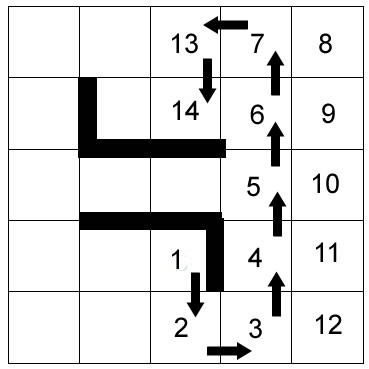
\includegraphics[width=200pt,height=200pt]{q1-dfs.jpg} }

\newpage

1.b) Uniform Cost Search

{\center 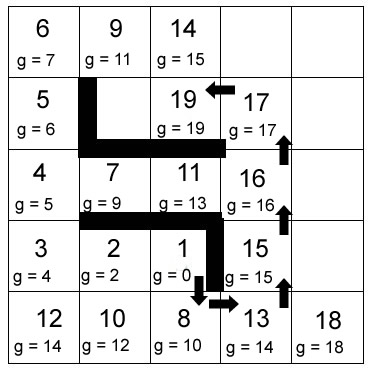
\includegraphics[width=200pt,height=200pt]{q1-ucs.jpg} }

\newpage

1.c) Greedy Best First Search

{\center 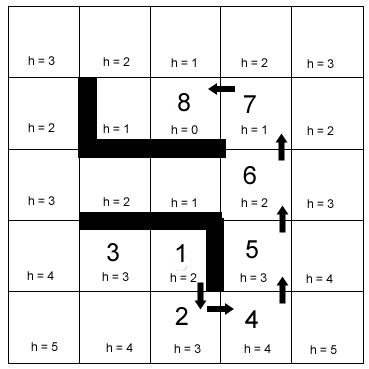
\includegraphics[width=200pt,height=200pt]{q1-gbfs.jpg} }

\newpage

1.d) $A^*$ Search

{\center 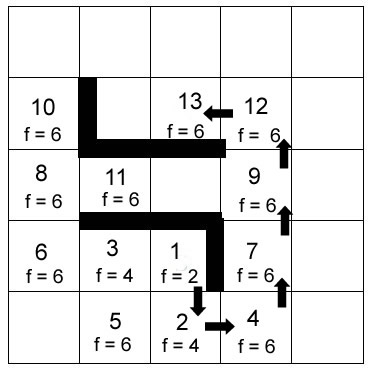
\includegraphics[width=200pt,height=200pt]{q1-astar.jpg} }

\newpage

2.a) At any point in time, we must know the locations of both the robots, so
our state description is $(\alpha,\beta)$ where $\alpha$ is the node in the
graph at which robot A is currently located, and $\beta$ is the node where
the robot B is located. The initial state in our state space is $(a,c)$ since
the robot A starts at node a, and the robot B starts at node c. Similarly the
goal state in our state space is $(b,d)$.

Let us define $shortestPath(x,y)$ to be the length of the shortest path from
node x to node y. Then a state $(\alpha,\beta)$ is {\it legal} if
$shortestPath(\alpha,\beta) \geq t$. Note that if $(a,c)$ and $(b,d)$ are not
legal, then there is trivially no solution.

For a given state $(\alpha,\beta)$, the set of legal next states is given by:
\begin{align*}
    \{ (\alpha',\beta) | \alpha' \text{ is a neighbor of } \alpha \text{ and } (\alpha',\beta) \text{ is legal.} \}
    \cup \\
    \{ (\alpha,\beta') | \beta'  \text{ is a neighbor of } \beta  \text{ and } (\alpha,\beta') \text{ is legal.} \}
\end{align*}

Since the building graph is static, the shortest path between each pair of nodes
can be precaculated and stored. The Floyd-Warshall algorithm can compute the
shortest paths for all pairs of nodes in $O(n^3)$ time, where $n$ is the number
of nodes in the graph. Checking if a state is legal can then be done in constant
time by looking up in the precalculated table.

2.b)Consider the following function:
\[ h(\alpha,\beta) = shortestPath(\alpha,b) + shortestPath(\beta,d). \]
When robot A is at position $\alpha$, it needs at least $shortestPath(\alpha,b)$
steps to reach the destination. Similarly robot B needs at least $shortestPath(\beta,d)$
steps to reach the goal. Since at each step only one robot can move, $h$ measures
the least number of steps required for both robots to reach their destinations.
Even the optimal solution cannot do better than this, so the $A^*$ criteria is met.

Note that our definition of $h$ doesn't incorporate $t$ at all. There is no simple
way we can incorporate $t$ into our heuristic, because while computing all pairs
shortest paths is easy, computing two paths such that they are always $t$ nodes 
apart is considerably harder.

\newpage

3.a) Minimax algorithm

{\center 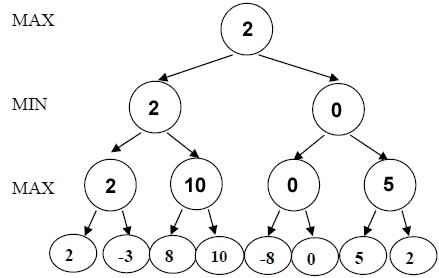
\includegraphics[width=300pt,height=180pt]{q3a.jpg} }

3.b) Alpha Beta Pruning

{\center 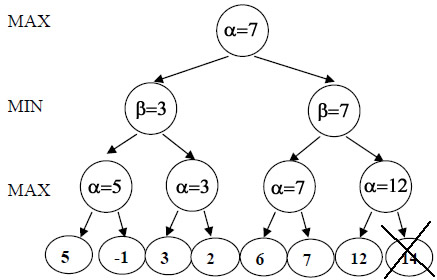
\includegraphics[width=300pt,height=180pt]{q3b.jpg} }

\newpage

4.1) Basic Alpha Beta Pruning Source Code

\lstinputlisting[frame=single]{../hw2/AlphaBetaPlayer.java}

\newpage

4.2) Static Board Evaluation function.

The value of a particular state of the board is calculated as follows. A positive
value implies advantage for the Red player, and a negative value for the Black player.

\begin{align*}
	value(B) &= (\sum_{r \in RED} value(r)) - (\sum_{b \in BLACK} value(b))
\end{align*}

where $value(B)$ is the value of the game, calculated as the difference between the collective
values of the Red and Black pieces. The value of each piece $value(p)$ is calculated as:
\begin{align*}
	value(p) = \begin{cases}
							10 + dof(p) + attacks(p) & \text{p is a pawn.}
							\cr
							25 + dof(p) + attacks(p) & \text{p is a king.}
						 \end{cases}
\end{align*}
Each of the terms is explained in more details below:
\begin{enumerate}
	\item Each piece has a \emph{base value}, which is chosen
		to be 10 for pawns and 25 for kings.
	\item $dof(p)$ measure the \emph{degree of freedom} each piece has. Note that
	  this measures the static freedom each piece has, not considering other pieces.
	  All it serves to do is to give piece in the middle of the board a slightly more
	  importance than those on the edges. For a pawn, this can be any of $\{0,1,2\}$, and
	  for a king $\{0,1,2,3,4\}$.
	\item $attacks(p)$ counts the number of pieces this piece can attack. It doesn't
		consider multiple jumps.For a pawn, this can be any of $\{0,1,2\}$, and
	  for a king $\{0,1,2,3,4\}$.
\end{enumerate}

To get an idea of the performance of this function against the basic one, 10 games were
played between the basic player and this implementation, with the evaluation function being
the only difference between the implementations. Out of 10, 6 games were won by the 
enhanced implementation, 3 by the basic one, and 1 game got stuck. To ensure that the
same games are not replayed, a small random component of $\pm 2$ was added to the 
evaluation function. This has a significant effect especially in the initial few moves
where the board is equally good for both players.

\emph{Strengths of implementation}: Favouring states which have higher attack potential is
a hueristic which works most of the time. We can think of this as an approximate
look-ahead into the next state, and counting how many next states will result in a 
enemy capture.

\emph{Weaknesses of implementation}: Since this is an approximate heuristic, we can always
find situations where this leads to a bad situation. Since the weights of the factors are
arbitrary, there is no statistical guarantee that this function will perform better than
any other implementation. In some situations, the weight given to attack potential is 
far too less, but in some other situations, it is too less, since in one move a piece can
attack only one other piece. Also, the degree of freedom should have weight much less than
attack potential in most cases, but there is no simple way of figuring out what the weight
should be.

The source code for the evaluation function is given below:

\begin{lstlisting}[frame=single]
protected int scoreCheckerBoard(int [][] bs,int whosTurn)
{
	int redValue = 0;
	int blackValue = 0;
	for(int i = 0 ; i < Utils.BOARD_WIDTH; ++i)
		for(int j = 0; j < Utils.BOARD_HEIGHT; ++j){
			switch(bs[i][j]){
				case RED_PAWN:
					redValue += 10; //base
					redValue += isValid(i-1,j-1) + isValid(i-1,j+1); //dof
					redValue += canAttack(bs,i - 1,j - 1, i - 2, j - 2, BLACK_PLAYER) +
								canAttack(bs,i - 1,j + 1, i - 2, j + 2, BLACK_PLAYER); //attacks
				break;
				case RED_KING:
					redValue += 25; //base
					redValue += isValid(i-1,j-1) + isValid(i-1,j+1) +
								isValid(i+1,j-1) + isValid(i+1,j+1); //dof
					redValue += canAttack(bs,i - 1,j - 1, i - 2, j - 2, BLACK_PLAYER) +
								canAttack(bs,i - 1,j + 1, i - 2, j + 2, BLACK_PLAYER) +
								canAttack(bs,i + 1,j - 1, i + 2, j - 2, BLACK_PLAYER) +
								canAttack(bs,i + 1,j + 1, i + 2, j + 2, BLACK_PLAYER); //attacks
				break;
				case BLACK_PAWN:
					blackValue += 10; //base
					blackValue += isValid(i+1,j-1) + isValid(i+1,j+1); //dof
					blackValue += canAttack(bs,i + 1,j - 1, i + 2, j - 2, RED_PLAYER) +
								  canAttack(bs,i + 1,j + 1, i + 2, j + 2, RED_PLAYER); //attacks
				break;
				case BLACK_KING:
					blackValue += 25;
					blackValue += isValid(i-1,j-1) + isValid(i-1,j+1) +
								  isValid(i+1,j-1) + isValid(i+1,j+1); //dof
					blackValue += canAttack(bs,i - 1,j - 1, i - 2, j - 2, RED_PLAYER) +
								  canAttack(bs,i - 1,j + 1, i - 2, j + 2, RED_PLAYER) +
								  canAttack(bs,i + 1,j - 1, i + 2, j - 2, RED_PLAYER) +
								  canAttack(bs,i + 1,j + 1, i + 2, j + 2, RED_PLAYER);//attacks
				break;
			}
		}
	return redValue - blackValue + ((int)(Math.random() * 4) - 2);
}
//returns 1 if the location is valid
private int isValid(int i,int j)
{
	if(i >= 0 && i < BOARD_WIDTH)
		if(j >= 0 && j < BOARD_HEIGHT)
			return 1;
	return 0;
}
//can i jump over enemy piece at (x1,y1) to empty location (x2,x2)
private int canAttack(int [][] bs,int x1, int y1, int x2, int y2, int otherPlayer)
{
	if(isValid(x1, y1) == 0 || isValid(x2, y2) == 0 ) return 0;
	if(Utils.getOwner(bs[x1][y1]) == otherPlayer && bs[x2][y2] == BLANK) return 1;
	return 0;
}
\end{lstlisting}

\end{document}